\documentclass[twoside]{book}

% Packages required by doxygen
\usepackage{fixltx2e}
\usepackage{calc}
\usepackage{doxygen}
\usepackage[export]{adjustbox} % also loads graphicx
\usepackage{graphicx}
\usepackage[utf8]{inputenc}
\usepackage{makeidx}
\usepackage{multicol}
\usepackage{multirow}
\PassOptionsToPackage{warn}{textcomp}
\usepackage{textcomp}
\usepackage[nointegrals]{wasysym}
\usepackage[table]{xcolor}

% Font selection
\usepackage[T1]{fontenc}
\usepackage[scaled=.90]{helvet}
\usepackage{courier}
\usepackage{amssymb}
\usepackage{sectsty}
\renewcommand{\familydefault}{\sfdefault}
\allsectionsfont{%
  \fontseries{bc}\selectfont%
  \color{darkgray}%
}
\renewcommand{\DoxyLabelFont}{%
  \fontseries{bc}\selectfont%
  \color{darkgray}%
}
\newcommand{\+}{\discretionary{\mbox{\scriptsize$\hookleftarrow$}}{}{}}

% Page & text layout
\usepackage{geometry}
\geometry{%
  a4paper,%
  top=2.5cm,%
  bottom=2.5cm,%
  left=2.5cm,%
  right=2.5cm%
}
\tolerance=750
\hfuzz=15pt
\hbadness=750
\setlength{\emergencystretch}{15pt}
\setlength{\parindent}{0cm}
\setlength{\parskip}{0.2cm}
\makeatletter
\renewcommand{\paragraph}{%
  \@startsection{paragraph}{4}{0ex}{-1.0ex}{1.0ex}{%
    \normalfont\normalsize\bfseries\SS@parafont%
  }%
}
\renewcommand{\subparagraph}{%
  \@startsection{subparagraph}{5}{0ex}{-1.0ex}{1.0ex}{%
    \normalfont\normalsize\bfseries\SS@subparafont%
  }%
}
\makeatother

% Headers & footers
\usepackage{fancyhdr}
\pagestyle{fancyplain}
\fancyhead[LE]{\fancyplain{}{\bfseries\thepage}}
\fancyhead[CE]{\fancyplain{}{}}
\fancyhead[RE]{\fancyplain{}{\bfseries\leftmark}}
\fancyhead[LO]{\fancyplain{}{\bfseries\rightmark}}
\fancyhead[CO]{\fancyplain{}{}}
\fancyhead[RO]{\fancyplain{}{\bfseries\thepage}}
\fancyfoot[LE]{\fancyplain{}{}}
\fancyfoot[CE]{\fancyplain{}{}}
\fancyfoot[RE]{\fancyplain{}{\bfseries\scriptsize Generated on Fri Aug 18 2017 20\+:45\+:46 for My Project by Doxygen }}
\fancyfoot[LO]{\fancyplain{}{\bfseries\scriptsize Generated on Fri Aug 18 2017 20\+:45\+:46 for My Project by Doxygen }}
\fancyfoot[CO]{\fancyplain{}{}}
\fancyfoot[RO]{\fancyplain{}{}}
\renewcommand{\footrulewidth}{0.4pt}
\renewcommand{\chaptermark}[1]{%
  \markboth{#1}{}%
}
\renewcommand{\sectionmark}[1]{%
  \markright{\thesection\ #1}%
}

% Indices & bibliography
\usepackage{natbib}
\usepackage[titles]{tocloft}
\setcounter{tocdepth}{3}
\setcounter{secnumdepth}{5}
\makeindex

% Hyperlinks (required, but should be loaded last)
\usepackage{ifpdf}
\ifpdf
  \usepackage[pdftex,pagebackref=true]{hyperref}
\else
  \usepackage[ps2pdf,pagebackref=true]{hyperref}
\fi
\hypersetup{%
  colorlinks=true,%
  linkcolor=blue,%
  citecolor=blue,%
  unicode%
}

% Custom commands
\newcommand{\clearemptydoublepage}{%
  \newpage{\pagestyle{empty}\cleardoublepage}%
}


%===== C O N T E N T S =====

\begin{document}

% Titlepage & ToC
\hypersetup{pageanchor=false,
             bookmarks=true,
             bookmarksnumbered=true,
             pdfencoding=unicode
            }
\pagenumbering{roman}
\begin{titlepage}
\vspace*{7cm}
\begin{center}%
{\Large My Project }\\
\vspace*{1cm}
{\large Generated by Doxygen 1.8.9.1}\\
\vspace*{0.5cm}
{\small Fri Aug 18 2017 20:45:46}\\
\end{center}
\end{titlepage}
\clearemptydoublepage
\tableofcontents
\clearemptydoublepage
\pagenumbering{arabic}
\hypersetup{pageanchor=true}

%--- Begin generated contents ---
\chapter{Namespace Index}
\section{Namespace List}
Here is a list of all documented namespaces with brief descriptions\+:\begin{DoxyCompactList}
\item\contentsline{section}{\hyperlink{namespace_dungeon_crawler}{Dungeon\+Crawler} }{\pageref{namespace_dungeon_crawler}}{}
\item\contentsline{section}{\hyperlink{namespace_dungeon_crawler_1_1_actions}{Dungeon\+Crawler.\+Actions} }{\pageref{namespace_dungeon_crawler_1_1_actions}}{}
\item\contentsline{section}{\hyperlink{namespace_dungeon_crawler_1_1_aspect}{Dungeon\+Crawler.\+Aspect} }{\pageref{namespace_dungeon_crawler_1_1_aspect}}{}
\item\contentsline{section}{\hyperlink{namespace_dungeon_crawler_1_1_character}{Dungeon\+Crawler.\+Character} }{\pageref{namespace_dungeon_crawler_1_1_character}}{}
\item\contentsline{section}{\hyperlink{namespace_dungeon_crawler_1_1_properties}{Dungeon\+Crawler.\+Properties} }{\pageref{namespace_dungeon_crawler_1_1_properties}}{}
\item\contentsline{section}{\hyperlink{namespace_dungeon_crawler_1_1_utilities}{Dungeon\+Crawler.\+Utilities} }{\pageref{namespace_dungeon_crawler_1_1_utilities}}{}
\end{DoxyCompactList}

\chapter{Hierarchical Index}
\section{Class Hierarchy}
This inheritance list is sorted roughly, but not completely, alphabetically\+:\begin{DoxyCompactList}
\item \contentsline{section}{Dungeon\+Crawler.\+Core.\+Aspect}{\pageref{class_dungeon_crawler_1_1_core_1_1_aspect}}{}
\item \contentsline{section}{Dungeon\+Crawler.\+Character.\+Attribute}{\pageref{class_dungeon_crawler_1_1_character_1_1_attribute}}{}
\item \contentsline{section}{Dungeon\+Crawler.\+Core.\+Cell}{\pageref{class_dungeon_crawler_1_1_core_1_1_cell}}{}
\item \contentsline{section}{Dungeon\+Crawler.\+Character.\+Character}{\pageref{class_dungeon_crawler_1_1_character_1_1_character}}{}
\item \contentsline{section}{Dungeon\+Crawler.\+Character.\+Consequence}{\pageref{class_dungeon_crawler_1_1_character_1_1_consequence}}{}
\item \contentsline{section}{Dungeon\+Crawler.\+Character.\+Inventory}{\pageref{class_dungeon_crawler_1_1_character_1_1_inventory}}{}
\item \contentsline{section}{Dungeon\+Crawler.\+Core.\+Item}{\pageref{class_dungeon_crawler_1_1_core_1_1_item}}{}
\begin{DoxyCompactList}
\item \contentsline{section}{Dungeon\+Crawler.\+Core.\+Armour}{\pageref{class_dungeon_crawler_1_1_core_1_1_armour}}{}
\item \contentsline{section}{Dungeon\+Crawler.\+Core.\+Weapon}{\pageref{class_dungeon_crawler_1_1_core_1_1_weapon}}{}
\end{DoxyCompactList}
\item \contentsline{section}{Dungeon\+Crawler.\+Core.\+Rulebook}{\pageref{class_dungeon_crawler_1_1_core_1_1_rulebook}}{}
\item \contentsline{section}{Dungeon\+Crawler.\+Core.\+Skill}{\pageref{class_dungeon_crawler_1_1_core_1_1_skill}}{}
\end{DoxyCompactList}

\chapter{Class Index}
\section{Class List}
Here are the classes, structs, unions and interfaces with brief descriptions\+:\begin{DoxyCompactList}
\item\contentsline{section}{\hyperlink{class_dungeon_crawler_1_1_aspect_1_1_aspect}{Dungeon\+Crawler.\+Aspect.\+Aspect} }{\pageref{class_dungeon_crawler_1_1_aspect_1_1_aspect}}{}
\item\contentsline{section}{\hyperlink{class_dungeon_crawler_1_1_actions_1_1_attack_action}{Dungeon\+Crawler.\+Actions.\+Attack\+Action} }{\pageref{class_dungeon_crawler_1_1_actions_1_1_attack_action}}{}
\item\contentsline{section}{\hyperlink{class_dungeon_crawler_1_1_character_1_1_attribute}{Dungeon\+Crawler.\+Character.\+Attribute} }{\pageref{class_dungeon_crawler_1_1_character_1_1_attribute}}{}
\item\contentsline{section}{\hyperlink{class_dungeon_crawler_1_1_character_1_1_character}{Dungeon\+Crawler.\+Character.\+Character} }{\pageref{class_dungeon_crawler_1_1_character_1_1_character}}{}
\item\contentsline{section}{\hyperlink{class_dungeon_crawler_1_1_character_1_1_consequence}{Dungeon\+Crawler.\+Character.\+Consequence} }{\pageref{class_dungeon_crawler_1_1_character_1_1_consequence}}{}
\item\contentsline{section}{\hyperlink{class_dungeon_crawler_1_1_items_1_1_item}{Dungeon\+Crawler.\+Items.\+Item} }{\pageref{class_dungeon_crawler_1_1_items_1_1_item}}{}
\item\contentsline{section}{\hyperlink{class_dungeon_crawler_1_1_items_1_1_item_database}{Dungeon\+Crawler.\+Items.\+Item\+Database} }{\pageref{class_dungeon_crawler_1_1_items_1_1_item_database}}{}
\item\contentsline{section}{\hyperlink{class_dungeon_crawler_1_1_aspect_1_1_tags_table}{Dungeon\+Crawler.\+Aspect.\+Tags\+Table} }{\pageref{class_dungeon_crawler_1_1_aspect_1_1_tags_table}}{}
\end{DoxyCompactList}

\chapter{Namespace Documentation}
\hypertarget{namespace_dungeon_crawler}{}\section{Package Dungeon\+Crawler}
\label{namespace_dungeon_crawler}\index{Dungeon\+Crawler@{Dungeon\+Crawler}}
\subsection*{Namespaces}
\begin{DoxyCompactItemize}
\item 
package \hyperlink{namespace_dungeon_crawler_1_1_actions}{Actions}
\item 
package \hyperlink{namespace_dungeon_crawler_1_1_aspect}{Aspect}
\item 
package \hyperlink{namespace_dungeon_crawler_1_1_character}{Character}
\item 
package \hyperlink{namespace_dungeon_crawler_1_1_properties}{Properties}
\item 
package \hyperlink{namespace_dungeon_crawler_1_1_utilities}{Utilities}
\end{DoxyCompactItemize}

\hypertarget{namespace_dungeon_crawler_1_1_character}{}\section{Package Dungeon\+Crawler.\+Character}
\label{namespace_dungeon_crawler_1_1_character}\index{Dungeon\+Crawler.\+Character@{Dungeon\+Crawler.\+Character}}
\subsection*{Classes}
\begin{DoxyCompactItemize}
\item 
class \hyperlink{class_dungeon_crawler_1_1_character_1_1_attribute}{Attribute}
\item 
class \hyperlink{class_dungeon_crawler_1_1_character_1_1_character}{Character}
\item 
class \hyperlink{class_dungeon_crawler_1_1_character_1_1_consequence}{Consequence}
\item 
class \hyperlink{class_dungeon_crawler_1_1_character_1_1_inventory}{Inventory}
\end{DoxyCompactItemize}

\hypertarget{namespace_dungeon_crawler_1_1_core}{}\section{Package Dungeon\+Crawler.\+Core}
\label{namespace_dungeon_crawler_1_1_core}\index{Dungeon\+Crawler.\+Core@{Dungeon\+Crawler.\+Core}}
\subsection*{Classes}
\begin{DoxyCompactItemize}
\item 
class \hyperlink{class_dungeon_crawler_1_1_core_1_1_armour}{Armour}
\item 
class \hyperlink{class_dungeon_crawler_1_1_core_1_1_aspect}{Aspect}
\item 
class \hyperlink{class_dungeon_crawler_1_1_core_1_1_cell}{Cell}
\item 
class {\bfseries Dice}
\item 
class {\bfseries Game\+Events\+Logger}
\item 
class {\bfseries Game\+Master}
\item 
class \hyperlink{class_dungeon_crawler_1_1_core_1_1_item}{Item}
\item 
class \hyperlink{class_dungeon_crawler_1_1_core_1_1_rulebook}{Rulebook}
\item 
class \hyperlink{class_dungeon_crawler_1_1_core_1_1_skill}{Skill}
\item 
class \hyperlink{class_dungeon_crawler_1_1_core_1_1_weapon}{Weapon}
\end{DoxyCompactItemize}

\hypertarget{namespace_dungeon_crawler_1_1_properties}{}\section{Package Dungeon\+Crawler.\+Properties}
\label{namespace_dungeon_crawler_1_1_properties}\index{Dungeon\+Crawler.\+Properties@{Dungeon\+Crawler.\+Properties}}
\subsection*{Classes}
\begin{DoxyCompactItemize}
\item 
class {\bfseries Settings}
\end{DoxyCompactItemize}

\chapter{Class Documentation}
\hypertarget{class_dungeon_crawler_1_1_core_1_1_armour}{}\section{Dungeon\+Crawler.\+Core.\+Armour Class Reference}
\label{class_dungeon_crawler_1_1_core_1_1_armour}\index{Dungeon\+Crawler.\+Core.\+Armour@{Dungeon\+Crawler.\+Core.\+Armour}}
Inheritance diagram for Dungeon\+Crawler.\+Core.\+Armour\+:\begin{figure}[H]
\begin{center}
\leavevmode
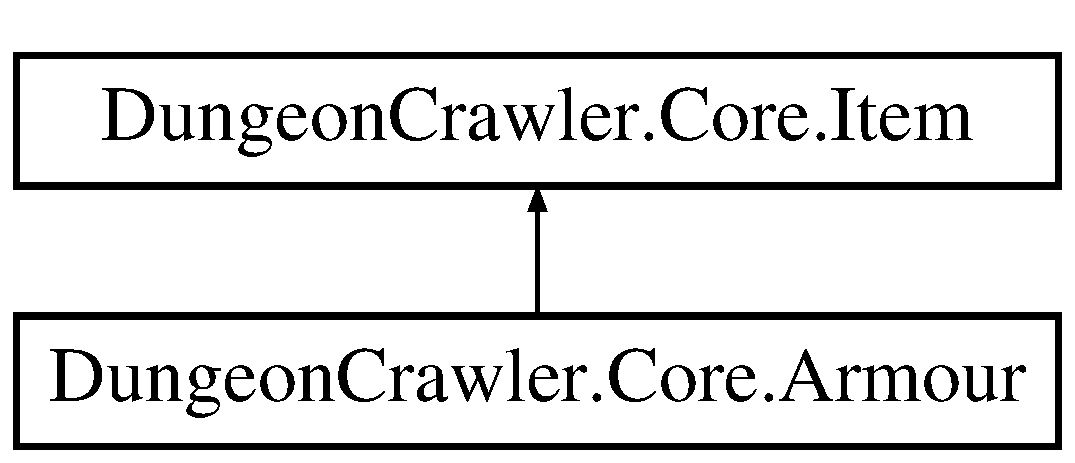
\includegraphics[height=2.000000cm]{class_dungeon_crawler_1_1_core_1_1_armour}
\end{center}
\end{figure}
\subsection*{Static Public Member Functions}
\begin{DoxyCompactItemize}
\item 
\hypertarget{class_dungeon_crawler_1_1_core_1_1_armour_a67a79103dade1a8fa1898c48c87a9cba}{}new static \hyperlink{class_dungeon_crawler_1_1_core_1_1_armour}{Armour} {\bfseries Deserialize\+From\+Json} (string json)\label{class_dungeon_crawler_1_1_core_1_1_armour_a67a79103dade1a8fa1898c48c87a9cba}

\end{DoxyCompactItemize}
\subsection*{Public Attributes}
\begin{DoxyCompactItemize}
\item 
\hypertarget{class_dungeon_crawler_1_1_core_1_1_armour_a9aeafda493381b0d102f92c66d70447f}{}int {\bfseries Protection}\label{class_dungeon_crawler_1_1_core_1_1_armour_a9aeafda493381b0d102f92c66d70447f}

\item 
\hypertarget{class_dungeon_crawler_1_1_core_1_1_armour_a4c12244c933ffdac443404a509daedd1}{}\hyperlink{class_dungeon_crawler_1_1_character_1_1_consequence}{Character.\+Consequence}\mbox{[}$\,$\mbox{]} {\bfseries Consequences}\label{class_dungeon_crawler_1_1_core_1_1_armour_a4c12244c933ffdac443404a509daedd1}

\end{DoxyCompactItemize}


The documentation for this class was generated from the following file\+:\begin{DoxyCompactItemize}
\item 
C\+:/projects/dungeoncrawler/cs/\+Dungeon\+Crawler/\+Core/Item.\+cs\end{DoxyCompactItemize}

\hypertarget{class_dungeon_crawler_1_1_core_1_1_aspect}{}\section{Dungeon\+Crawler.\+Core.\+Aspect Class Reference}
\label{class_dungeon_crawler_1_1_core_1_1_aspect}\index{Dungeon\+Crawler.\+Core.\+Aspect@{Dungeon\+Crawler.\+Core.\+Aspect}}
\subsection*{Public Member Functions}
\begin{DoxyCompactItemize}
\item 
\hypertarget{class_dungeon_crawler_1_1_core_1_1_aspect_a6205fbdf664eb5ec8955fd4576e5c503}{}{\bfseries Aspect} (string name, string\mbox{[}$\,$\mbox{]} skills, int bonus)\label{class_dungeon_crawler_1_1_core_1_1_aspect_a6205fbdf664eb5ec8955fd4576e5c503}

\item 
\hypertarget{class_dungeon_crawler_1_1_core_1_1_aspect_ab392c10aea5ca423c735d02a98ec4846}{}int {\bfseries Matches} (string\mbox{[}$\,$\mbox{]} tags)\label{class_dungeon_crawler_1_1_core_1_1_aspect_ab392c10aea5ca423c735d02a98ec4846}

\end{DoxyCompactItemize}
\subsection*{Public Attributes}
\begin{DoxyCompactItemize}
\item 
\hypertarget{class_dungeon_crawler_1_1_core_1_1_aspect_a34928312abdb48beae781b348e1b6d40}{}string {\bfseries Name}\label{class_dungeon_crawler_1_1_core_1_1_aspect_a34928312abdb48beae781b348e1b6d40}

\item 
\hypertarget{class_dungeon_crawler_1_1_core_1_1_aspect_a7f9cede50bd9f13359cf5d0c4b9e68d4}{}string\mbox{[}$\,$\mbox{]} {\bfseries Skills}\label{class_dungeon_crawler_1_1_core_1_1_aspect_a7f9cede50bd9f13359cf5d0c4b9e68d4}

\item 
\hypertarget{class_dungeon_crawler_1_1_core_1_1_aspect_a0dedd71fade2cc68e95d8145638145f9}{}int {\bfseries Bonus}\label{class_dungeon_crawler_1_1_core_1_1_aspect_a0dedd71fade2cc68e95d8145638145f9}

\item 
\hypertarget{class_dungeon_crawler_1_1_core_1_1_aspect_a4f275f0e7a11ed65fa69115a7200a757}{}string\mbox{[}$\,$\mbox{]} {\bfseries Tags}\label{class_dungeon_crawler_1_1_core_1_1_aspect_a4f275f0e7a11ed65fa69115a7200a757}

\end{DoxyCompactItemize}
\subsection*{Properties}
\begin{DoxyCompactItemize}
\item 
\hypertarget{class_dungeon_crawler_1_1_core_1_1_aspect_afef3ab7f16fca5563a025e7dcf720cc9}{}int {\bfseries Cost}\hspace{0.3cm}{\ttfamily  \mbox{[}get\mbox{]}}\label{class_dungeon_crawler_1_1_core_1_1_aspect_afef3ab7f16fca5563a025e7dcf720cc9}

\end{DoxyCompactItemize}


The documentation for this class was generated from the following file\+:\begin{DoxyCompactItemize}
\item 
C\+:/projects/dungeoncrawler/cs/\+Dungeon\+Crawler/\+Core/Aspect.\+cs\end{DoxyCompactItemize}

\hypertarget{class_dungeon_crawler_1_1_character_1_1_attribute}{}\section{Dungeon\+Crawler.\+Character.\+Attribute Class Reference}
\label{class_dungeon_crawler_1_1_character_1_1_attribute}\index{Dungeon\+Crawler.\+Character.\+Attribute@{Dungeon\+Crawler.\+Character.\+Attribute}}
\subsection*{Public Member Functions}
\begin{DoxyCompactItemize}
\item 
\hypertarget{class_dungeon_crawler_1_1_character_1_1_attribute_ab72a00669748ae0d34854e204f6c2bc3}{}{\bfseries Attribute} (int value, int max\+Value, int min\+Value)\label{class_dungeon_crawler_1_1_character_1_1_attribute_ab72a00669748ae0d34854e204f6c2bc3}

\end{DoxyCompactItemize}
\subsection*{Public Attributes}
\begin{DoxyCompactItemize}
\item 
\hypertarget{class_dungeon_crawler_1_1_character_1_1_attribute_a6b90a26a21371fb4ef9be0f59e0969d4}{}int {\bfseries Value}\label{class_dungeon_crawler_1_1_character_1_1_attribute_a6b90a26a21371fb4ef9be0f59e0969d4}

\item 
\hypertarget{class_dungeon_crawler_1_1_character_1_1_attribute_ada64988d817204be249a826ef2397505}{}int {\bfseries Max\+Value}\label{class_dungeon_crawler_1_1_character_1_1_attribute_ada64988d817204be249a826ef2397505}

\item 
\hypertarget{class_dungeon_crawler_1_1_character_1_1_attribute_ad3948aff878c3e156284f58af0fb0783}{}int {\bfseries Min\+Value}\label{class_dungeon_crawler_1_1_character_1_1_attribute_ad3948aff878c3e156284f58af0fb0783}

\end{DoxyCompactItemize}


The documentation for this class was generated from the following file\+:\begin{DoxyCompactItemize}
\item 
C\+:/projects/dungeoncrawler/cs/\+Dungeon\+Crawler/\+Character/Character.\+cs\end{DoxyCompactItemize}

\hypertarget{class_dungeon_crawler_1_1_core_1_1_cell}{}\section{Dungeon\+Crawler.\+Core.\+Cell Class Reference}
\label{class_dungeon_crawler_1_1_core_1_1_cell}\index{Dungeon\+Crawler.\+Core.\+Cell@{Dungeon\+Crawler.\+Core.\+Cell}}
\subsection*{Public Attributes}
\begin{DoxyCompactItemize}
\item 
\hypertarget{class_dungeon_crawler_1_1_core_1_1_cell_aa3d2bdde1e93cc3604f3aa1d915eeae7}{}string\mbox{[}$\,$\mbox{]} {\bfseries Tags}\label{class_dungeon_crawler_1_1_core_1_1_cell_aa3d2bdde1e93cc3604f3aa1d915eeae7}

\end{DoxyCompactItemize}


The documentation for this class was generated from the following file\+:\begin{DoxyCompactItemize}
\item 
C\+:/projects/dungeoncrawler/cs/\+Dungeon\+Crawler/\+Core/Cell.\+cs\end{DoxyCompactItemize}

\hypertarget{class_dungeon_crawler_1_1_character_1_1_character}{}\section{Dungeon\+Crawler.\+Character.\+Character Class Reference}
\label{class_dungeon_crawler_1_1_character_1_1_character}\index{Dungeon\+Crawler.\+Character.\+Character@{Dungeon\+Crawler.\+Character.\+Character}}
\subsection*{Public Member Functions}
\begin{DoxyCompactItemize}
\item 
\hypertarget{class_dungeon_crawler_1_1_character_1_1_character_a60ed0daf6e2a281318dc35effe82566c}{}void {\bfseries Equip} (string item\+Name, string slot)\label{class_dungeon_crawler_1_1_character_1_1_character_a60ed0daf6e2a281318dc35effe82566c}

\item 
\hypertarget{class_dungeon_crawler_1_1_character_1_1_character_a625216059f7c3d1dfa61bd93ac32c8be}{}void {\bfseries Un\+Equip} (string item\+Name)\label{class_dungeon_crawler_1_1_character_1_1_character_a625216059f7c3d1dfa61bd93ac32c8be}

\item 
\hypertarget{class_dungeon_crawler_1_1_character_1_1_character_a497e5dede14b0215ee42f96b7dbba3f5}{}\hyperlink{class_dungeon_crawler_1_1_aspect_1_1_aspect}{Aspect.\+Aspect}\mbox{[}$\,$\mbox{]} {\bfseries Aspects\+Affecting\+Skill} (string skill)\label{class_dungeon_crawler_1_1_character_1_1_character_a497e5dede14b0215ee42f96b7dbba3f5}

\item 
\hypertarget{class_dungeon_crawler_1_1_character_1_1_character_ac7a76a986b94456d8bc1e11ce3ca1fb0}{}int {\bfseries Skill\+Value} (string skill, string\mbox{[}$\,$\mbox{]} tags)\label{class_dungeon_crawler_1_1_character_1_1_character_ac7a76a986b94456d8bc1e11ce3ca1fb0}

\item 
\hypertarget{class_dungeon_crawler_1_1_character_1_1_character_ae055249e1c6ee3731014f8f65f5ab93e}{}void {\bfseries Take\+Physical\+Damage} (int shifts)\label{class_dungeon_crawler_1_1_character_1_1_character_ae055249e1c6ee3731014f8f65f5ab93e}

\item 
\hypertarget{class_dungeon_crawler_1_1_character_1_1_character_a33b3dc221862864ee9ace0323e3c1ce4}{}void {\bfseries Take\+Consequence} (int shifts)\label{class_dungeon_crawler_1_1_character_1_1_character_a33b3dc221862864ee9ace0323e3c1ce4}

\end{DoxyCompactItemize}
\subsection*{Static Public Member Functions}
\begin{DoxyCompactItemize}
\item 
\hypertarget{class_dungeon_crawler_1_1_character_1_1_character_afa98f6089012bcc1077fbae13e6abfd5}{}static \hyperlink{class_dungeon_crawler_1_1_character_1_1_character}{Character} {\bfseries Deserialize\+From\+Json} (string json)\label{class_dungeon_crawler_1_1_character_1_1_character_afa98f6089012bcc1077fbae13e6abfd5}

\item 
\hypertarget{class_dungeon_crawler_1_1_character_1_1_character_a0e4ae66b1518972809a7e41a59b0be36}{}static string {\bfseries Serialize\+To\+Json} (\hyperlink{class_dungeon_crawler_1_1_character_1_1_character}{Character} character)\label{class_dungeon_crawler_1_1_character_1_1_character_a0e4ae66b1518972809a7e41a59b0be36}

\end{DoxyCompactItemize}
\subsection*{Public Attributes}
\begin{DoxyCompactItemize}
\item 
\hypertarget{class_dungeon_crawler_1_1_character_1_1_character_aa2d1b857beb2c58f0c38f094c50e637c}{}int {\bfseries Id}\label{class_dungeon_crawler_1_1_character_1_1_character_aa2d1b857beb2c58f0c38f094c50e637c}

\item 
\hypertarget{class_dungeon_crawler_1_1_character_1_1_character_abb90f6709fba71190b636ab3fce18d27}{}string {\bfseries Name}\label{class_dungeon_crawler_1_1_character_1_1_character_abb90f6709fba71190b636ab3fce18d27}

\item 
\hypertarget{class_dungeon_crawler_1_1_character_1_1_character_ae1fd66371018c048b20507a58ca45289}{}\hyperlink{class_dungeon_crawler_1_1_character_1_1_attribute}{Attribute} {\bfseries Physical\+Stress}\label{class_dungeon_crawler_1_1_character_1_1_character_ae1fd66371018c048b20507a58ca45289}

\item 
\hypertarget{class_dungeon_crawler_1_1_character_1_1_character_ad7ee68985ab5bfca6b632d7aff45e6bf}{}List$<$ \hyperlink{class_dungeon_crawler_1_1_character_1_1_consequence}{Consequence} $>$ {\bfseries Consequences}\label{class_dungeon_crawler_1_1_character_1_1_character_ad7ee68985ab5bfca6b632d7aff45e6bf}

\item 
\hypertarget{class_dungeon_crawler_1_1_character_1_1_character_a93a18c279d78d511e25d73260110962a}{}Dictionary$<$ string, int $>$ {\bfseries Skills}\label{class_dungeon_crawler_1_1_character_1_1_character_a93a18c279d78d511e25d73260110962a}

\item 
\hypertarget{class_dungeon_crawler_1_1_character_1_1_character_a552a419b69680243d8243ba5959a90bf}{}string\mbox{[}$\,$\mbox{]} {\bfseries Tags}\label{class_dungeon_crawler_1_1_character_1_1_character_a552a419b69680243d8243ba5959a90bf}

\item 
\hypertarget{class_dungeon_crawler_1_1_character_1_1_character_a45cfcdcc9191e3a08aaef402ff979eb4}{}List$<$ \hyperlink{class_dungeon_crawler_1_1_aspect_1_1_aspect}{Aspect.\+Aspect} $>$ {\bfseries Aspects}\label{class_dungeon_crawler_1_1_character_1_1_character_a45cfcdcc9191e3a08aaef402ff979eb4}

\item 
\hypertarget{class_dungeon_crawler_1_1_character_1_1_character_a22cda9a13deb74dd0089970150354c9b}{}Dictionary$<$ string, string $>$ {\bfseries Equipment}\label{class_dungeon_crawler_1_1_character_1_1_character_a22cda9a13deb74dd0089970150354c9b}

\item 
\hypertarget{class_dungeon_crawler_1_1_character_1_1_character_aa9be269eb8ea184174ad9e27e06638e7}{}bool {\bfseries Is\+Taken\+Out}\label{class_dungeon_crawler_1_1_character_1_1_character_aa9be269eb8ea184174ad9e27e06638e7}

\end{DoxyCompactItemize}
\subsection*{Properties}
\begin{DoxyCompactItemize}
\item 
\hypertarget{class_dungeon_crawler_1_1_character_1_1_character_a9ad914f0cc7420b7450f780fe8b46a53}{}List$<$ \hyperlink{class_dungeon_crawler_1_1_aspect_1_1_aspect}{Aspect.\+Aspect} $>$ {\bfseries All\+Aspects}\hspace{0.3cm}{\ttfamily  \mbox{[}get\mbox{]}}\label{class_dungeon_crawler_1_1_character_1_1_character_a9ad914f0cc7420b7450f780fe8b46a53}

\end{DoxyCompactItemize}


The documentation for this class was generated from the following file\+:\begin{DoxyCompactItemize}
\item 
C\+:/projects/dungeoncrawler/cs/\+Dungeon\+Crawler/\+Character/Character.\+cs\end{DoxyCompactItemize}

\hypertarget{class_dungeon_crawler_1_1_character_1_1_consequence}{}\section{Dungeon\+Crawler.\+Character.\+Consequence Class Reference}
\label{class_dungeon_crawler_1_1_character_1_1_consequence}\index{Dungeon\+Crawler.\+Character.\+Consequence@{Dungeon\+Crawler.\+Character.\+Consequence}}
\subsection*{Public Member Functions}
\begin{DoxyCompactItemize}
\item 
\hypertarget{class_dungeon_crawler_1_1_character_1_1_consequence_ad8642b949789aaea7d22e38f6b3778dd}{}{\bfseries Consequence} (string name, int capacity, bool is\+Taken=false, \hyperlink{class_dungeon_crawler_1_1_core_1_1_aspect}{Aspect} effect=null)\label{class_dungeon_crawler_1_1_character_1_1_consequence_ad8642b949789aaea7d22e38f6b3778dd}

\item 
\hypertarget{class_dungeon_crawler_1_1_character_1_1_consequence_ad9944b48d59878f68d5339ba5add1db5}{}void {\bfseries Take} ()\label{class_dungeon_crawler_1_1_character_1_1_consequence_ad9944b48d59878f68d5339ba5add1db5}

\end{DoxyCompactItemize}
\subsection*{Public Attributes}
\begin{DoxyCompactItemize}
\item 
\hypertarget{class_dungeon_crawler_1_1_character_1_1_consequence_a0b0cf26945a8efb3402b955098693b47}{}string {\bfseries Name}\label{class_dungeon_crawler_1_1_character_1_1_consequence_a0b0cf26945a8efb3402b955098693b47}

\item 
\hypertarget{class_dungeon_crawler_1_1_character_1_1_consequence_ab6931c76cc48bf013f71a7128df9decf}{}int {\bfseries Capacity}\label{class_dungeon_crawler_1_1_character_1_1_consequence_ab6931c76cc48bf013f71a7128df9decf}

\item 
\hypertarget{class_dungeon_crawler_1_1_character_1_1_consequence_ab01e2cf751dff41dc90dd550991e8dda}{}bool {\bfseries Is\+Taken}\label{class_dungeon_crawler_1_1_character_1_1_consequence_ab01e2cf751dff41dc90dd550991e8dda}

\item 
\hypertarget{class_dungeon_crawler_1_1_character_1_1_consequence_aef0467da62c63e37bf27527dded9871f}{}\hyperlink{class_dungeon_crawler_1_1_core_1_1_aspect}{Aspect} {\bfseries Effect}\label{class_dungeon_crawler_1_1_character_1_1_consequence_aef0467da62c63e37bf27527dded9871f}

\end{DoxyCompactItemize}


The documentation for this class was generated from the following file\+:\begin{DoxyCompactItemize}
\item 
C\+:/projects/dungeoncrawler/cs/\+Dungeon\+Crawler/\+Character/Character.\+cs\end{DoxyCompactItemize}

\hypertarget{class_dungeon_crawler_1_1_character_1_1_inventory}{}\section{Dungeon\+Crawler.\+Character.\+Inventory Class Reference}
\label{class_dungeon_crawler_1_1_character_1_1_inventory}\index{Dungeon\+Crawler.\+Character.\+Inventory@{Dungeon\+Crawler.\+Character.\+Inventory}}
\subsection*{Public Member Functions}
\begin{DoxyCompactItemize}
\item 
\hypertarget{class_dungeon_crawler_1_1_character_1_1_inventory_af5584f56326553ac8150b49f9e631b7d}{}void {\bfseries Add\+Item} (\hyperlink{class_dungeon_crawler_1_1_core_1_1_item}{Item} item, int amount=1)\label{class_dungeon_crawler_1_1_character_1_1_inventory_af5584f56326553ac8150b49f9e631b7d}

\item 
\hypertarget{class_dungeon_crawler_1_1_character_1_1_inventory_a6c885ad8274da8c39787744b44c9bfde}{}\hyperlink{class_dungeon_crawler_1_1_core_1_1_item}{Item} {\bfseries Item} (string name)\label{class_dungeon_crawler_1_1_character_1_1_inventory_a6c885ad8274da8c39787744b44c9bfde}

\item 
\hypertarget{class_dungeon_crawler_1_1_character_1_1_inventory_a3fb85209eba0aca801458a6b690679bc}{}void {\bfseries Remove\+Item} (\hyperlink{class_dungeon_crawler_1_1_core_1_1_item}{Item} item, int amount=1)\label{class_dungeon_crawler_1_1_character_1_1_inventory_a3fb85209eba0aca801458a6b690679bc}

\end{DoxyCompactItemize}
\subsection*{Public Attributes}
\begin{DoxyCompactItemize}
\item 
\hypertarget{class_dungeon_crawler_1_1_character_1_1_inventory_a470eb7828ae32ab8702a671d41812bb1}{}List$<$ \hyperlink{class_dungeon_crawler_1_1_core_1_1_item}{Item} $>$ {\bfseries Items}\label{class_dungeon_crawler_1_1_character_1_1_inventory_a470eb7828ae32ab8702a671d41812bb1}

\item 
\hypertarget{class_dungeon_crawler_1_1_character_1_1_inventory_ac1ce6fd154f4dcf2fdefd89db2a1f28e}{}List$<$ \hyperlink{class_dungeon_crawler_1_1_core_1_1_weapon}{Weapon} $>$ {\bfseries Weapons}\label{class_dungeon_crawler_1_1_character_1_1_inventory_ac1ce6fd154f4dcf2fdefd89db2a1f28e}

\item 
\hypertarget{class_dungeon_crawler_1_1_character_1_1_inventory_a61b8d31b7b04ae4fe1d0f6adb4cdfcaf}{}List$<$ \hyperlink{class_dungeon_crawler_1_1_core_1_1_armour}{Armour} $>$ {\bfseries Armours}\label{class_dungeon_crawler_1_1_character_1_1_inventory_a61b8d31b7b04ae4fe1d0f6adb4cdfcaf}

\item 
\hypertarget{class_dungeon_crawler_1_1_character_1_1_inventory_a1c1ead94848b857ac163c6e820370d5f}{}Dictionary$<$ string, int $>$ {\bfseries Amounts}\label{class_dungeon_crawler_1_1_character_1_1_inventory_a1c1ead94848b857ac163c6e820370d5f}

\end{DoxyCompactItemize}


The documentation for this class was generated from the following file\+:\begin{DoxyCompactItemize}
\item 
C\+:/projects/dungeoncrawler/cs/\+Dungeon\+Crawler/\+Character/Inventory.\+cs\end{DoxyCompactItemize}

\hypertarget{class_dungeon_crawler_1_1_core_1_1_item}{}\section{Dungeon\+Crawler.\+Core.\+Item Class Reference}
\label{class_dungeon_crawler_1_1_core_1_1_item}\index{Dungeon\+Crawler.\+Core.\+Item@{Dungeon\+Crawler.\+Core.\+Item}}
Inheritance diagram for Dungeon\+Crawler.\+Core.\+Item\+:\begin{figure}[H]
\begin{center}
\leavevmode
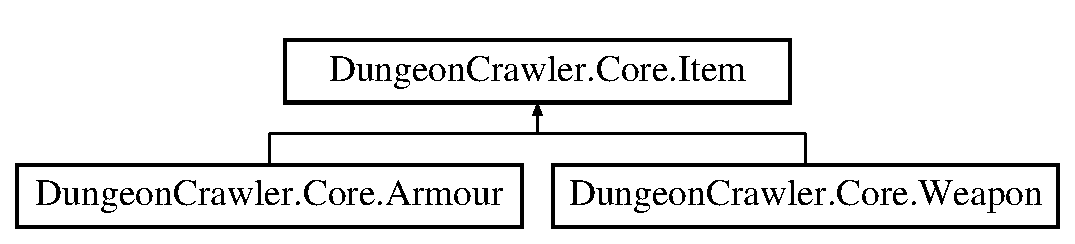
\includegraphics[height=2.000000cm]{class_dungeon_crawler_1_1_core_1_1_item}
\end{center}
\end{figure}
\subsection*{Static Public Member Functions}
\begin{DoxyCompactItemize}
\item 
\hypertarget{class_dungeon_crawler_1_1_core_1_1_item_a22c805fd74054dc453cc8710b7b0a023}{}static \hyperlink{class_dungeon_crawler_1_1_core_1_1_item}{Item} {\bfseries Deserialize\+From\+Json} (string json)\label{class_dungeon_crawler_1_1_core_1_1_item_a22c805fd74054dc453cc8710b7b0a023}

\end{DoxyCompactItemize}
\subsection*{Public Attributes}
\begin{DoxyCompactItemize}
\item 
\hypertarget{class_dungeon_crawler_1_1_core_1_1_item_ab24f9d839ae3b24d3dbbceffa8617764}{}string {\bfseries Name}\label{class_dungeon_crawler_1_1_core_1_1_item_ab24f9d839ae3b24d3dbbceffa8617764}

\item 
\hypertarget{class_dungeon_crawler_1_1_core_1_1_item_af11c39625f65ca6261e749a9d4119c61}{}\hyperlink{class_dungeon_crawler_1_1_core_1_1_aspect}{Aspect}\mbox{[}$\,$\mbox{]} {\bfseries Aspects}\label{class_dungeon_crawler_1_1_core_1_1_item_af11c39625f65ca6261e749a9d4119c61}

\item 
\hypertarget{class_dungeon_crawler_1_1_core_1_1_item_a9b5424ecb05cba5b5e96db05de4bf71e}{}string\mbox{[}$\,$\mbox{]} {\bfseries Tags}\label{class_dungeon_crawler_1_1_core_1_1_item_a9b5424ecb05cba5b5e96db05de4bf71e}

\item 
\hypertarget{class_dungeon_crawler_1_1_core_1_1_item_a6d0c7b4ba5b26317ec7b5491f0f03501}{}string {\bfseries Equipment\+Slot}\label{class_dungeon_crawler_1_1_core_1_1_item_a6d0c7b4ba5b26317ec7b5491f0f03501}

\end{DoxyCompactItemize}


The documentation for this class was generated from the following file\+:\begin{DoxyCompactItemize}
\item 
C\+:/projects/dungeoncrawler/cs/\+Dungeon\+Crawler/\+Core/Item.\+cs\end{DoxyCompactItemize}

\hypertarget{class_dungeon_crawler_1_1_core_1_1_rulebook}{}\section{Dungeon\+Crawler.\+Core.\+Rulebook Class Reference}
\label{class_dungeon_crawler_1_1_core_1_1_rulebook}\index{Dungeon\+Crawler.\+Core.\+Rulebook@{Dungeon\+Crawler.\+Core.\+Rulebook}}
\subsection*{Static Public Member Functions}
\begin{DoxyCompactItemize}
\item 
\hypertarget{class_dungeon_crawler_1_1_core_1_1_rulebook_a8421b5449b51ff2de2256f88414b94db}{}static string\mbox{[}$\,$\mbox{]} {\bfseries Synonyms\+Of} (string tag)\label{class_dungeon_crawler_1_1_core_1_1_rulebook_a8421b5449b51ff2de2256f88414b94db}

\item 
\hypertarget{class_dungeon_crawler_1_1_core_1_1_rulebook_af8f68a06d3cc955b5251c26e4c21cb6b}{}static \hyperlink{class_dungeon_crawler_1_1_core_1_1_item}{Item} {\bfseries Item} (string name)\label{class_dungeon_crawler_1_1_core_1_1_rulebook_af8f68a06d3cc955b5251c26e4c21cb6b}

\item 
\hypertarget{class_dungeon_crawler_1_1_core_1_1_rulebook_a4567b47de0202da43ce45b8868681cd1}{}static \hyperlink{class_dungeon_crawler_1_1_core_1_1_weapon}{Weapon} {\bfseries Weapon} (string name)\label{class_dungeon_crawler_1_1_core_1_1_rulebook_a4567b47de0202da43ce45b8868681cd1}

\item 
\hypertarget{class_dungeon_crawler_1_1_core_1_1_rulebook_a36372fc256493e580b7745312d6bd41b}{}static \hyperlink{class_dungeon_crawler_1_1_core_1_1_armour}{Armour} {\bfseries Armour} (string name)\label{class_dungeon_crawler_1_1_core_1_1_rulebook_a36372fc256493e580b7745312d6bd41b}

\item 
\hypertarget{class_dungeon_crawler_1_1_core_1_1_rulebook_ad07da757abd45ca3e99c18be74ee845f}{}static void {\bfseries Deserialize\+From\+Json} (string json)\label{class_dungeon_crawler_1_1_core_1_1_rulebook_ad07da757abd45ca3e99c18be74ee845f}

\item 
\hypertarget{class_dungeon_crawler_1_1_core_1_1_rulebook_a9885764a9561d091f425316042987e8b}{}static string {\bfseries Serialize\+To\+Json} ()\label{class_dungeon_crawler_1_1_core_1_1_rulebook_a9885764a9561d091f425316042987e8b}

\end{DoxyCompactItemize}
\subsection*{Public Attributes}
\begin{DoxyCompactItemize}
\item 
\hypertarget{class_dungeon_crawler_1_1_core_1_1_rulebook_afff9e91efa6e6581f7b02b4baeb5e756}{}Dictionary$<$ string, \hyperlink{class_dungeon_crawler_1_1_core_1_1_skill}{Skill} $>$ {\bfseries Skills} = new Dictionary$<$string, \hyperlink{class_dungeon_crawler_1_1_core_1_1_skill}{Skill}$>$()\label{class_dungeon_crawler_1_1_core_1_1_rulebook_afff9e91efa6e6581f7b02b4baeb5e756}

\item 
\hypertarget{class_dungeon_crawler_1_1_core_1_1_rulebook_acd5fb3739084cde354ae4d729354fbe3}{}Dictionary$<$ string, string\mbox{[}$\,$\mbox{]}$>$ {\bfseries Tags} = new Dictionary$<$string, string\mbox{[}$\,$\mbox{]}$>$()\label{class_dungeon_crawler_1_1_core_1_1_rulebook_acd5fb3739084cde354ae4d729354fbe3}

\item 
\hypertarget{class_dungeon_crawler_1_1_core_1_1_rulebook_a56af8e1641ddce45fa078dade8aec12e}{}List$<$ \hyperlink{class_dungeon_crawler_1_1_core_1_1_item}{Item} $>$ {\bfseries Items} = new List$<$\hyperlink{class_dungeon_crawler_1_1_core_1_1_item}{Item}$>$()\label{class_dungeon_crawler_1_1_core_1_1_rulebook_a56af8e1641ddce45fa078dade8aec12e}

\item 
\hypertarget{class_dungeon_crawler_1_1_core_1_1_rulebook_a636bdadcc92b81c2f8d427bce718128f}{}List$<$ \hyperlink{class_dungeon_crawler_1_1_core_1_1_weapon}{Weapon} $>$ {\bfseries Weapons} = new List$<$\hyperlink{class_dungeon_crawler_1_1_core_1_1_weapon}{Weapon}$>$()\label{class_dungeon_crawler_1_1_core_1_1_rulebook_a636bdadcc92b81c2f8d427bce718128f}

\item 
\hypertarget{class_dungeon_crawler_1_1_core_1_1_rulebook_a4885fa840e4fb2bdc585aa1d9f135169}{}List$<$ \hyperlink{class_dungeon_crawler_1_1_core_1_1_armour}{Armour} $>$ {\bfseries Armours} = new List$<$\hyperlink{class_dungeon_crawler_1_1_core_1_1_armour}{Armour}$>$()\label{class_dungeon_crawler_1_1_core_1_1_rulebook_a4885fa840e4fb2bdc585aa1d9f135169}

\end{DoxyCompactItemize}
\subsection*{Properties}
\begin{DoxyCompactItemize}
\item 
\hypertarget{class_dungeon_crawler_1_1_core_1_1_rulebook_a113e93268afaa03eb3d7c0ce9ef284e7}{}static \hyperlink{class_dungeon_crawler_1_1_core_1_1_rulebook}{Rulebook} {\bfseries Instance}\hspace{0.3cm}{\ttfamily  \mbox{[}get, set\mbox{]}}\label{class_dungeon_crawler_1_1_core_1_1_rulebook_a113e93268afaa03eb3d7c0ce9ef284e7}

\end{DoxyCompactItemize}


The documentation for this class was generated from the following file\+:\begin{DoxyCompactItemize}
\item 
C\+:/projects/dungeoncrawler/cs/\+Dungeon\+Crawler/\+Core/Rulebook.\+cs\end{DoxyCompactItemize}

\hypertarget{class_dungeon_crawler_1_1_core_1_1_skill}{}\section{Dungeon\+Crawler.\+Core.\+Skill Class Reference}
\label{class_dungeon_crawler_1_1_core_1_1_skill}\index{Dungeon\+Crawler.\+Core.\+Skill@{Dungeon\+Crawler.\+Core.\+Skill}}
\subsection*{Public Attributes}
\begin{DoxyCompactItemize}
\item 
\hypertarget{class_dungeon_crawler_1_1_core_1_1_skill_ace8f3c8fa159d45483f754bf53654ee7}{}string {\bfseries Name}\label{class_dungeon_crawler_1_1_core_1_1_skill_ace8f3c8fa159d45483f754bf53654ee7}

\item 
\hypertarget{class_dungeon_crawler_1_1_core_1_1_skill_a52e0bd49a51f220a30d7c59c30712434}{}string {\bfseries Description}\label{class_dungeon_crawler_1_1_core_1_1_skill_a52e0bd49a51f220a30d7c59c30712434}

\item 
\hypertarget{class_dungeon_crawler_1_1_core_1_1_skill_abf3d93fafabca6f964357707de5dac15}{}string\mbox{[}$\,$\mbox{]} {\bfseries Opposing\+Skills}\label{class_dungeon_crawler_1_1_core_1_1_skill_abf3d93fafabca6f964357707de5dac15}

\item 
\hypertarget{class_dungeon_crawler_1_1_core_1_1_skill_a8b622ec466f07a5e50ba891f48188e71}{}string\mbox{[}$\,$\mbox{]} {\bfseries Actions}\label{class_dungeon_crawler_1_1_core_1_1_skill_a8b622ec466f07a5e50ba891f48188e71}

\end{DoxyCompactItemize}


The documentation for this class was generated from the following file\+:\begin{DoxyCompactItemize}
\item 
C\+:/projects/dungeoncrawler/cs/\+Dungeon\+Crawler/\+Core/Skill.\+cs\end{DoxyCompactItemize}

\hypertarget{class_dungeon_crawler_1_1_core_1_1_weapon}{}\section{Dungeon\+Crawler.\+Core.\+Weapon Class Reference}
\label{class_dungeon_crawler_1_1_core_1_1_weapon}\index{Dungeon\+Crawler.\+Core.\+Weapon@{Dungeon\+Crawler.\+Core.\+Weapon}}
Inheritance diagram for Dungeon\+Crawler.\+Core.\+Weapon\+:\begin{figure}[H]
\begin{center}
\leavevmode
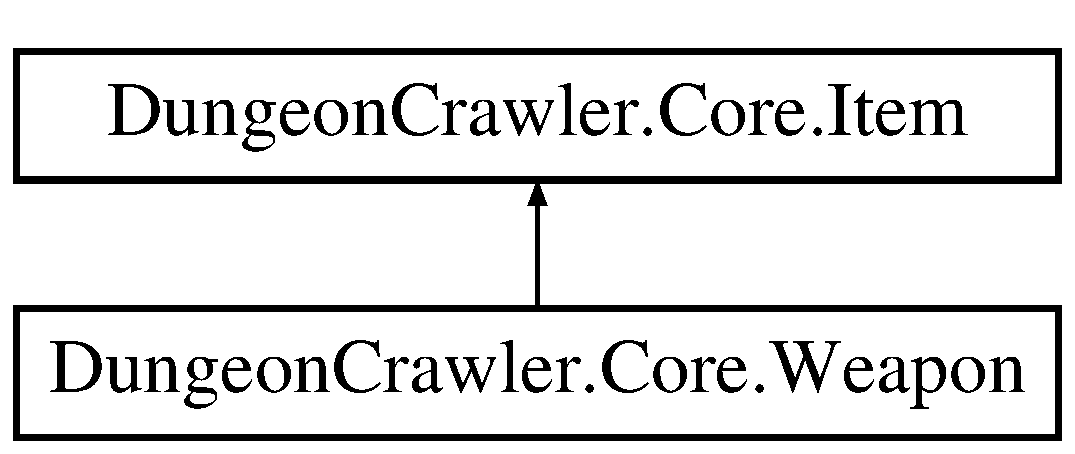
\includegraphics[height=2.000000cm]{class_dungeon_crawler_1_1_core_1_1_weapon}
\end{center}
\end{figure}
\subsection*{Static Public Member Functions}
\begin{DoxyCompactItemize}
\item 
\hypertarget{class_dungeon_crawler_1_1_core_1_1_weapon_a6d99de4da4b070ee5e5dbeef5e5f7481}{}new static \hyperlink{class_dungeon_crawler_1_1_core_1_1_weapon}{Weapon} {\bfseries Deserialize\+From\+Json} (string json)\label{class_dungeon_crawler_1_1_core_1_1_weapon_a6d99de4da4b070ee5e5dbeef5e5f7481}

\end{DoxyCompactItemize}
\subsection*{Public Attributes}
\begin{DoxyCompactItemize}
\item 
\hypertarget{class_dungeon_crawler_1_1_core_1_1_weapon_a320a9cc5a44478e81ce852b88557f03d}{}string\mbox{[}$\,$\mbox{]} {\bfseries Skills}\label{class_dungeon_crawler_1_1_core_1_1_weapon_a320a9cc5a44478e81ce852b88557f03d}

\item 
\hypertarget{class_dungeon_crawler_1_1_core_1_1_weapon_a2638db696abeed45dc2327e7c0e1e7ea}{}int {\bfseries Damage}\label{class_dungeon_crawler_1_1_core_1_1_weapon_a2638db696abeed45dc2327e7c0e1e7ea}

\end{DoxyCompactItemize}
\subsection*{Properties}
\begin{DoxyCompactItemize}
\item 
\hypertarget{class_dungeon_crawler_1_1_core_1_1_weapon_a2a4b8d41a1a3d9acf71ac55ccbf4556c}{}override int {\bfseries Cost}\hspace{0.3cm}{\ttfamily  \mbox{[}get\mbox{]}}\label{class_dungeon_crawler_1_1_core_1_1_weapon_a2a4b8d41a1a3d9acf71ac55ccbf4556c}

\end{DoxyCompactItemize}


The documentation for this class was generated from the following file\+:\begin{DoxyCompactItemize}
\item 
C\+:/projects/dungeoncrawler/cs/\+Dungeon\+Crawler/\+Core/Item.\+cs\end{DoxyCompactItemize}

%--- End generated contents ---

% Index
\backmatter
\newpage
\phantomsection
\clearemptydoublepage
\addcontentsline{toc}{chapter}{Index}
\printindex

\end{document}
